\lab{Discrete Fourier Transform}{Discrete Fourier Transform}
\objective{The analysis of periodic functions has many applications in pure and applied mathematics, especially in settings dealing with sound waves. The Fourier transform provides a way to analyze such periodic functions. In this lab, we implement the discrete Fourier transform and explore digital audio signals in Python.}

\section*{Sound Waves}

Sounds are vibrations in the air around us.
The frequency and intensity of these vibrations determine how sound is perceived.
Sounds correspond physically to continuous functions, but they may be discretely approximated on a computer.
These discrete approximations can be made indistinguishable from a continuous signal.

\section*{Digital Audio Signals}

There are two components of a digital audio signal: samples from the soundwave and a sample rate.
These correspond to the amplitude and frequency, respectively.
A sample is a measurement of the amplitude of the wave at an instant in time.
To see why the sample rate is necessary, consider an array with samples from a soundwave.
If we do not know how frequently those samples were collected then we can arbitrarily stretch or compress the soundwave to make a variety of sounds.
See Figure \ref{fig:comp_wave} for an illustration of this principle.

\begin{center}
\begin{figure}
\caption{A picture of samples from a soundwave with varything frequencies.  It should be stretched or compressed to show how the frequency changes. Also describe how the sounds would be perceived.  The stretched out signal will sound deeper-ish.  Liiiiikkkkeeee tttthhhhhiiiiissss.  The shorter one will sound higher-ish. Like this.}
\label{fig:comp_wave}
\end{figure}
\end{center}

However, if we know at what rate the samples were taken, then we can construct the wave exactly as it was recorded.
In most applications, this sample rate will be measured in number of samples taken per second.
The standard rate for high quality audio is $44100$ equally spaced samples per second.

% Problem 1: Signal class.
\begin{problem}
Write a class called \li{Signal} that creates a digital audio signal when instantiated.
The constructor should accept a sample rate (an integer) and an array of samples (a NumPy array).
Store these inputs as attributes.

Add a method to the class called \li{plot} that generates the graph of the soundwave (just plot the array of samples). % TODO: is this correct?
%Though the array of samples have the $y$-values of the soundwave, the $x$-values need to be calculated using the sample rate. %(?)

%Finally, implement the \li{__add__} magic method so that if two instances of \li{Signal} of the same length are added together, the sum of their signals are returned.% (as a new Signal object).
\end{problem}

\subsection*{Wave File Format} 

One of the most common audio file formats across operating systems is the \li{wave} format, also called \li{wav} after its file extension.
It is a lightweight, common standard that is in wide use.
SciPy has builtin tools to read and create \li{wav} files.
To read in a \li{wav} file, we can use the \li{read} function that returns the file's sample rate and samples.

\begin{lstlisting}
>>> from scipy.io import wavfile
>>> rate, signal = wavfile.read('tada.wav')
\end{lstlisting}

To get an idea of what the soundwave looks like, we plot \li{signal}.
See Figure \ref{fig:tada_sig}.

\begin{figure}[ht]\centering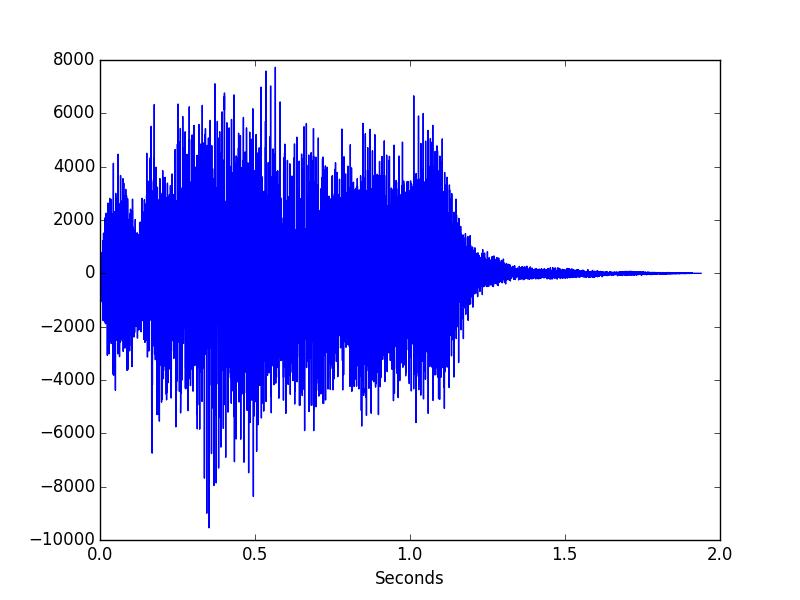
\includegraphics[width=\textwidth]{tada.png}\caption{The soundwave of \li{tada.wav}.}\label{fig:tada_sig}\end{figure}

For example, if we had a NumPy array called \li{signal}, we could create an audio file using the \li{write} method in the \li{scipy.io.wavfile} library.

\begin{lstlisting}
# Write a random signal sampled at a rate of 44100 hz to my_sound.wav.
>>> signal = np.random.randint(-32767, 32767, 30000)
>>> samplerate = 44100
>>> wavfile.write('my_sound.wav', samplerate, signal)
\end{lstlisting}

It should be noted that \li{wavfile.write} expects an array of 16 bit integers for the samples (whole numbers between $-32767$ and $32767$).
Therefore, waves may need to be scaled and converted to integers before using this function.

\begin{problem}

Add a method to the \li{Signal} class called \li{write_to_file} that generates a \li{.wav} file from the \li{signal} attribute.
The \li{write_to_file} method should accept the name of the file to be written.

\end{problem}

\section*{Creating Sounds in Python}

In order to generate a sound in python, we need to sample the corresponding sine wave and then save it as an audio file.
This can be done quite efficiently using \li{numpy} arrays and functions.
For example, suppose that we want to generate a sound with a frequency of 500 hertz for 10 seconds.
%We can use \li{numpy}'s \li{sin} function to generate the correct wave form.

\begin{lstlisting}
>>> samplerate = 44100
>>> frequency = 500
>>> length = 10         # Length in seconds of the desired sound.
\end{lstlisting}

Recall the the function $\sin(x)$ has a period of $2\pi$.
To create sounds, however, we want the period of our wave to be $1$, corresponding to $1$ second.
Thus, we will sample from the function
\[
\sin(2\pi xf)
\]
where $f$ is our desired frequency.
%# Create a lambda function to sample from.
%>>> wave_function = lambda x: np.sin(2*np.pi*x*frequency)
\begin{lstlisting}
>>> def wave_function(x):
...     return np.sin(2*np.pi*x*frequency)
\end{lstlisting}

In the following code, we generate a signal using three steps: first, find the correct step given the \li{samplerate}.
Next, generate the points at which we wish to sample the wave.
Finally, get the samples we want by passing \li{sample_points} to \li{wave_function}.

\begin{lstlisting}
>>> stepsize = 1./ samplerate
>>> sample_points = np.arange(0, length, stepsize)
>>> samples = wave_function(sample_points)
\end{lstlisting}

Our samples will be numbers between 0 to 1 taken from \li{wave_function}.
Recall that \li{wavfile.write} requires integeres between $-32767$ and $32767$.
Thus, we scale our sample points before creating a \li{.wav} file that can be played by the computer.

\begin{lstlisting}
>>> scaled_samples = np.int16(samples*32767)
\end{lstlisting}

The \li{scaled_samples} array can now be written to a file using \li{wavfile.write}.
This file can be played using media software included with most operating systems.

% Problem 3
\begin{problem}

The `A' note occurs at a frequency of 440 hertz.
Generate the sine wave that corresponds to an `A' note being played for 5 seconds.

Once you have successfully generated the `A' note, experiment with different frequencies to generate different notes.
The following table shows some frequencies that correspond to common notes.

\begin{center}
\begin{tabular}{|c|c|}
\hline
Note & Frequency \\
\hline
A & 440 \\
B & 493.88 \\
C & 523.25 \\
D & 587.33 \\
E & 659.25 \\
F & 698.46 \\
G & 783.99 \\
\hline
\end{tabular}
\end{center}

\end{problem}

\section*{Discrete Fourier Transform}

\subsection*{Some Technicalities}

Recall that under the right conditions, a continuous periodic function may be represented as a sum of sine waves:
\[
f(x) = \displaystyle{\sum_{k=-\infty}^{\infty}} c_k \sin{kx}
\]
where the constants $c_k$ are called the Fourier coefficients.

Further recall that such a transform also exists for discrete periodic functions.
Whereas the frequencies present in the continuous case are multiples of a sine wave with a period of 1, the discrete case is somewhat different.
The Fourier coefficients in the discrete case represent the amplitudes of sine waves whose periods are multiples of a ``fundamental frequency.''
The fundamental frequency is a sine wave with a period length equal to the amount of time of the signal.

The k$th$ coefficient of a signal $\{x_0, .., x_{N-1}\}$ is calculated with the following formula:
\[
c_k = \displaystyle{\sum_{n=0}^{N-1}} x_n \cdot e^{\frac{2\pi ikn}{N}}
\]
where $i$ is the square root of $-1$.
This process is done for each $k$ from $0$ to $N-1$.
Thus there are just as many Fourier coefficients as samples from the orginal signal.

% Problem 4
\begin{problem}

Add a method the \li{Signal} class called \li{calculate_DFT} that calculates the discrete Fourier transform of the \li{wave} attribute.
Store the calculated coefficients in an attribute called \li{DFT}.

The \li{scipy} module has a \li{fft} method that also calculates the discrete Fourier transform of an array.
Time the speed of your implmentation with the one in SciPy.
\end{problem}

% Fast fourier transform?

\section*{Plotting the DFT}

The graph of the fourier transform of a sound file is useful in applications.
While the graph of the original signal gives information about the amplitude of a soundwave at certain points, the graph of the discrete Fourier transform will show which frequencies are present in the signal.
For example, the sounds that we generated in the previous section contained only one frequency.
If we created an `A' note at 440 hz, then the graph of the DFT would appear as in Figure \ref{fig:dft_a}.

\begin{center}
\begin{figure}
\caption{The discrete Fourier transform of an `A' note.  Notice that there is only one spike in the graph, as there is only one frequency present.}
\label{fig:dft_a}
\end{figure}
\end{center}

On the other hand, the DFT of a more complicated soundwave will have many frequencies present.
See Figure \ref{fig:dft_tada} for an example.

\begin{center}
\begin{figure}
\caption{The discrete Fourier transform of \li{tada.wav}.  Each spike in the graph corresponds to a frequency that is present in the signal.}
\label{fig:dft_tada}
\end{figure}
\end{center} 

% Problem 5
\begin{problem}

Update the \li{plot} method so that it includes a kew word argument, \li{DFT}, that defaults to \li{False}.
If the \li{DFT} attribute is set to \li{True} by the user, then \li{plot} should generate a plot of the coefficients from the discrete Fourier transform.
If it is set to \li{False}, then the functionality should be unchanged.

\end{problem}

% Problem 6
\begin{problem}

A chord is a conjunction of several notes played together.
We may create a chord in python by adding several sound waves together.
For example, to create a chord with `A', `C', and `E' notes, we would generate the sound waves for each, as in the prior problem, and then add them together.
\begin{lstlisting}
# Create an A, C, and E note as before, and call them a_note, c_note, and e_note
chord = a_note + c_note + e_note
\end{lstlisting}

Create several chords and observe the plot of their DFT.
There should be as many spikes as there are notes in the plot.

Now, create a sound that changes over time.
(Hint: Start with a single note or chord and append another)
Examine the plot of the DFT.
How many frequencies are present?  Why?

\end{problem}

